\documentclass[border=8pt]{standalone}
\usepackage[T1]{fontenc}
\usepackage{mathptmx}
\usepackage{tikz}
\usetikzlibrary{arrows.meta,positioning,fit,calc,shapes.geometric,shapes.misc,shapes.multipart,backgrounds}
\tikzset{
  arr/.style={-{Stealth[length=2.4mm,width=1.8mm]},line width=0.6pt},
  box/.style={draw,line width=0.6pt,align=center,rounded corners=2pt},
}

\begin{document}
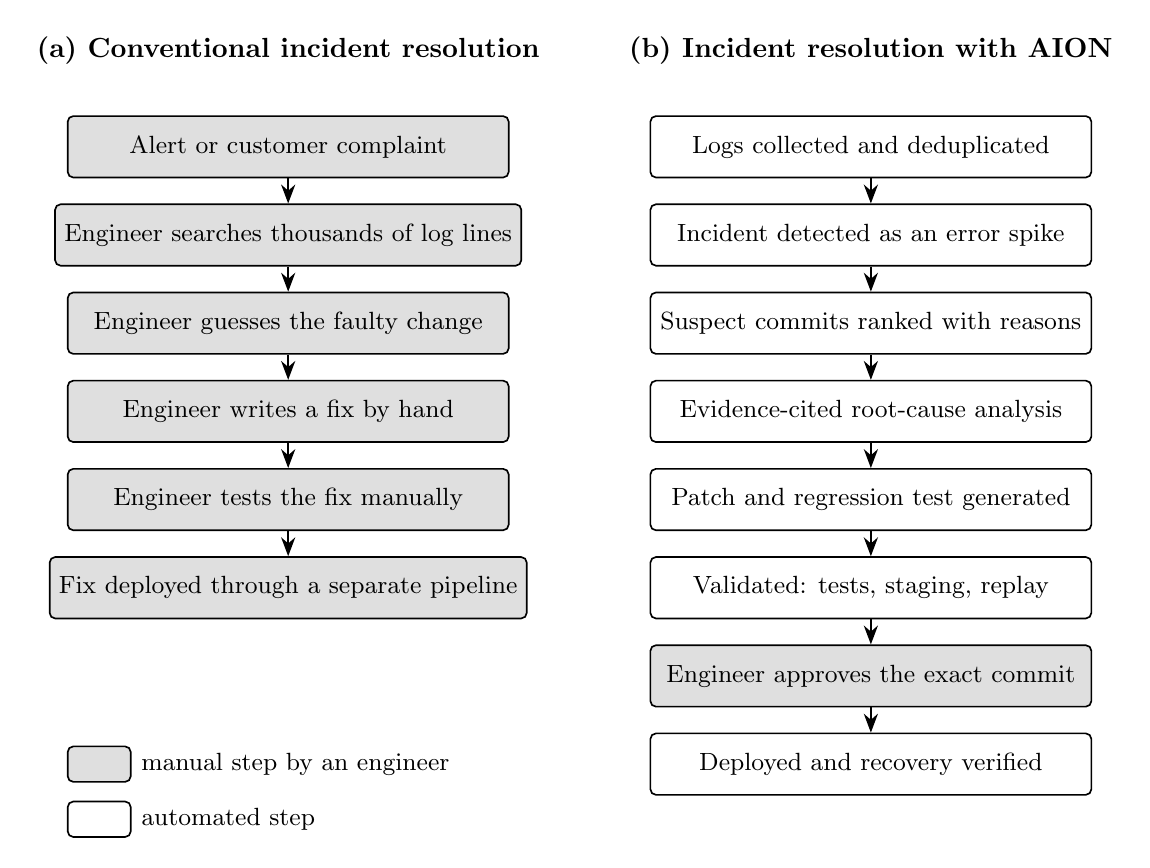
\begin{tikzpicture}[font=\small, b/.style={box, minimum width=5.6cm, minimum height=0.78cm}, m/.style={b, fill=gray!25}]
\node[font=\bfseries] at (0,0.1) {(a) Conventional incident resolution};
\node[font=\bfseries] at (7.4,0.1) {(b) Incident resolution with AION};
\foreach \t [count=\i] in {Alert or customer complaint, Engineer searches thousands of log lines, Engineer guesses the faulty change, Engineer writes a fix by hand, Engineer tests the fix manually, Fix deployed through a separate pipeline}{
  \node[m] (c\i) at (0,-\i*1.12) {\t};}
\foreach \i [evaluate=\i as \j using int(\i+1)] in {1,...,5}{\draw[arr] (c\i)--(c\j);}
\foreach \t [count=\i] in {Logs collected and deduplicated, Incident detected as an error spike, Suspect commits ranked with reasons, Evidence-cited root-cause analysis, Patch and regression test generated, {Validated: tests, staging, replay}}{
  \node[b] (a\i) at (7.4,-\i*1.12) {\t};}
\node[m] (a7) at (7.4,-7*1.12) {Engineer approves the exact commit};
\node[b] (a8) at (7.4,-8*1.12) {Deployed and recovery verified};
\foreach \i [evaluate=\i as \j using int(\i+1)] in {1,...,7}{\draw[arr] (a\i)--(a\j);}
\node[m, minimum width=0.8cm, minimum height=0.45cm] (l1) at (-2.4,-8.96) {};
\node[anchor=west] at (l1.east) {manual step by an engineer};
\node[b, minimum width=0.8cm, minimum height=0.45cm] (l2) at (-2.4,-9.66) {};
\node[anchor=west] at (l2.east) {automated step};
\end{tikzpicture}
\end{document}
